\documentclass[11pt,a4paper]{article}

% --- PACKAGES ---
\usepackage[utf8]{inputenc}
\usepackage[T1]{fontenc}
\usepackage[margin=2.0cm]{geometry}
\usepackage{amsmath,amssymb}
\usepackage{booktabs}
\usepackage{multirow}
\usepackage{xcolor}
\usepackage{tikz}
\usetikzlibrary{shapes.geometric, arrows.meta, positioning, shadows, calc, fit}
\usepackage{hyperref}
\usepackage{fancyhdr}
\usepackage{enumitem}
\usepackage{parskip}
\usepackage{pdflscape}
\usepackage[most]{tcolorbox}
\usepackage{tabularx}
\usepackage{graphicx}

% --- FIX HEADHEIGHT & TOPMARGIN FOR FANCYHDR ---
\setlength{\headheight}{14.0pt}
\addtolength{\topmargin}{-2.0pt}

% --- CUSTOM COLOR PALETTE ---
\definecolor{GoldPrimary}{HTML}{D4AF37}
\definecolor{GoldDark}{HTML}{9E7808}
\definecolor{DarkBG}{HTML}{1A1A1F}
\definecolor{CardBG}{HTML}{FFFFFF}
\definecolor{TealAccent}{HTML}{1B7A6E}
\definecolor{PurpleAccent}{HTML}{7D3C98}
\definecolor{RustAccent}{HTML}{D35400}
\definecolor{GreenAccent}{HTML}{229954}
\definecolor{BlueAccent}{HTML}{1F618D}
\definecolor{TextDark}{HTML}{1C2833}

% --- 10 FACET COLOR FINGERPRINT PALETTE ---
\definecolor{pF1}{HTML}{4BA6A6}
\definecolor{pF2}{HTML}{8AC926}
\definecolor{pF3}{HTML}{FFCA3A}
\definecolor{pF4}{HTML}{1982C4}
\definecolor{pF5}{HTML}{9B51E0}
\definecolor{pF6}{HTML}{2A9D8F}
\definecolor{pF7}{HTML}{E76F51}
\definecolor{pF8}{HTML}{52B788}
\definecolor{pF9}{HTML}{F77F00}
\definecolor{pF10}{HTML}{D4AF37}

% --- TCOLORBOX STYLES (SOLID HIGH-CONTRAST BANNERS) ---
\tcbset{
    boxrule=1.0pt,
    arc=4pt,
    fonttitle=\bfseries\small,
    colback=white,
    coltext=TextDark,
    boxsep=5pt,
    left=8pt,
    right=8pt
}

\newtcolorbox{sensoryquote}[1][]{
    enhanced,
    colback=white,
    colframe=GoldDark,
    colbacktitle=GoldDark,
    coltitle=white,
    fonttitle=\bfseries\small,
    title=SENSORY ILLUSION \& TACTILE PROFILE,
    fontupper=\itshape\color{TextDark},
    #1
}

\newtcolorbox{botanicalbox}[1][]{
    enhanced,
    colback=white,
    colframe=TealAccent,
    colbacktitle=TealAccent,
    coltitle=white,
    fonttitle=\bfseries\small,
    title=BOTANICAL ORIGIN \& ANATOMICAL FUNCTION,
    fontupper=\color{TextDark},
    #1
}

\newtcolorbox{flavourbox}[1][]{
    enhanced,
    colback=white,
    colframe=PurpleAccent,
    colbacktitle=PurpleAccent,
    coltitle=white,
    fonttitle=\bfseries\small,
    title=PALATE \& SENSORY FLAVOR EXPERIENCE,
    fontupper=\color{TextDark},
    #1
}

% --- HYPERREF SETUP ---
\hypersetup{
    colorlinks=true,
    linkcolor=GoldDark,
    citecolor=TealAccent,
    urlcolor=GoldDark,
    pdftitle={Deconstructing Fruit Architecture: The 10-Facet Masterclass Specification},
    pdfauthor={Perfumery Student Organ Suite}
}

% --- HEADER & FOOTER SETUP ---
\pagestyle{fancy}
\fancyhf{}
\rhead{\textcolor{GoldDark}{\small Deconstructing Fruit Architecture: 10-Facet Map}}
\lhead{\small\textcolor{gray}{Perfumery Course --- Phase 4}}
\rfoot{\small Page \thepage}

\begin{document}

% ==========================================
% TITLE BLOCK
% ==========================================
\begin{center}
    {\huge \bfseries \textcolor{GoldDark}{DECONSTRUCTING FRUIT ARCHITECTURE}}\\[0.4em]
    {\Large \bfseries The 10-Facet Botanical Lifecycle Map \& Master \texorpdfstring{10$\times$10}{10x10} Archetype Matrix}\\[0.8em]
    {\large \textcolor{gray}{A Structural Physical Chemistry Approach to Living Fruit Realism in Fine Fragrance}}\\[1.2em]
    \rule{\textwidth}{1.2pt}\\[1.5em]
\end{center}

\begin{abstract}
Traditional fruity fragrance formulation relies on simplified, flat ester mixtures (e.g., Ethyl Butanoate, Isoamyl Acetate) that yield synthetic "candy-like" impressions. This paper establishes the \textbf{3D Anatomical Lifecycle Model}, a comprehensive structural framework mapping living fruit anatomy across 10 distinct facets---from the outer epicarp wax ($F_1$) to inner mesocarp pith ($F_2$), fleshy core pulp ($F_3$), cytoplasmic vacuole sap ($F_4$), translucent aril ($F_5$), stem latex ($F_6$), lignified seed stone ($F_7$), calyx crown ($F_8$), and post-harvest thermal transformations ($F_9, F_{10}$). Integrating physical chemistry parameters---Vapor Pressure ($\text{VP}$ in $\text{Pa}$ at 25$^\circ$C), molecular weight ($\text{MW}$), and human odor thresholds ($\text{ppb}$)---with high-impact aroma chemicals, we provide the definitive \textbf{Master \texorpdfstring{10$\times$10}{10x10} Fruit Archetype Matrix} and compounding protocols for compounding hyper-realistic living fruit accords.
\end{abstract}

\vspace{1em}

% ==========================================
% SECTION 1: PHYSICAL CHEMISTRY & BIOCHEMISTRY
% ==========================================
\section{Physical Chemistry \& Plant Biochemistry of Fruit Realism}

Traditional perfumery training categorizes fruit notes into a simple top-note pyramid. However, headspace Gas Chromatography-Mass Spectrometry (GC-MS) analysis of living attached fruit shows that natural fruit aroma is a dynamic, multi-layered physical and biochemical matrix.

\subsection{Mathematical Model of Evaporative Flux}
The spatial evaporation of volatile compounds from living fruit tissue is governed by Raoult's Law modified for activity coefficients ($\gamma_i$) in aqueous-lipid cellular matrices:
\begin{equation}
    \text{Flux}_i(t) = \text{VP}_i \cdot \gamma_i \cdot x_i \cdot e^{-k_i t}
\end{equation}
where $\text{VP}_i$ represents pure substance vapor pressure at 25$^\circ$C (in $\text{Pa}$), $x_i$ is the mole fraction within the anatomical layer, and $k_i$ is the volatility decay constant.

\subsection{Biosynthetic Pathways \& Enzymatic Cascades}
Living fruit volatiles are generated via five primary plant biochemical pathways:
\begin{enumerate}[leftmargin=1.5em]
    \item \textbf{The Lipoxygenase (LOX) Pathway ($F_1, F_4, F_8$):} Polyunsaturated fatty acids (Linoleic $18:2$ and Linolenic $18:3$) undergo oxidation by Lipoxygenase (LOX) to form 13-hydroperoxides, which Hydroperoxide Lyase (HPL) cleaves into green $C_6$ aldehydes: Hexanal ($F_1$), cis-3-Hexenal, and (E)-2-Hexenal ($F_1$, \texttt{4GA02582}). Alcohol Dehydrogenase (ADH) reduces these into cis-3-Hexenol ($F_4$), which Alcohol Acyltransferase (AAT) esterifies into cis-3-Hexenyl Acetate ($F_8$).
    \item \textbf{Branched-Chain Amino Acid (BCAA) Transamination ($F_3, F_9$):} L-Isoleucine, L-Leucine, and L-Valine are converted by branched-chain aminotransferases (BCAT) and decarboxylases into acyl-CoA precursors, producing fruity esters like Ethyl 2-Methylbutanoate ($F_3$) and Isoamyl Acetate ($F_9$).
    \item \textbf{Phenylalanine Ammonia-Lyase (PAL) Pathway ($F_3, F_7$):} L-Phenylalanine is converted via the shikimate/PAL pathway into cyanic aromatic volatiles including Benzaldehyde ($F_7$), Benzyl Acetate ($F_3$), and Methyl Cinnamate.
    \item \textbf{Mevalonate / MEP Terpenoid Pathway ($F_1, F_5, F_6$):} Plastidial MEP pathways synthesize monoterpenes (d-Limonene, Myrcene, Terpinolene) and cyclic ethers (cis-Rose Oxide $F_5$) from Geranyl Diphosphate (GPP).
    \item \textbf{Carotenoid Cleavage (CCD) Pathway ($F_{10}$):} Carotenoid Cleavage Dioxygenases (CCDs) enzymatically degrade $\beta$-carotene and neoxanthin into high-impact norisoprenoids: $\beta$-Ionone ($F_{10}$, threshold $7\text{ ppt}$) and (E)-$\beta$-Damascenone ($F_{10}$, threshold $0.002\text{ ppb}$).
\end{enumerate}

\vspace{1em}

% ==========================================
% SECTION 2: TOPOLOGICAL LIFECYCLE FLOW
% ==========================================
\section{Topological Lifecycle Flow \& Evaporative Kinetics}

The term \textbf{"Topological"} refers to the structural spatial adjacency and non-linear degradation pathways connecting living plant tissues, rather than static Euclidean distance. Figure \ref{fig:lifecycle} maps these 10 facets across two fundamental axes: \textbf{Spatial Anatomical Layering} ($F_1 \rightarrow F_8$) and \textbf{Temporal Degradation Pathways} ($F_9, F_{10}$).

\subsection{1. Spatial Anatomical Adjacency ($F_1 \rightarrow F_8$)}
In living botany, volatile synthesis is localized in concentric tissue zones:
\begin{itemize}[leftmargin=1.5em]
    \item \textbf{Exocarp Skin ($F_1$):} Hydrophobic lipid wax layer harboring $C_6/C_{10}$ aldehydes and terpene hydrocarbons.
    \item \textbf{Mesocarp Albedo ($F_2$):} Cellulosic spongy pith containing pyrazines and green alcohols that provide bitter structural friction.
    \item \textbf{Core Parenchyma ($F_3, F_4$):} Fleshy pulp and vacuole water containing short-chain aliphatic esters ($1,700\text{ Pa}$) and melon/cucumber aldehydes.
    \item \textbf{Seed Aril \& Pit ($F_5, F_7$):} Mucilage envelopes rich in volatile thiols ($18\text{ Pa}$) enclosing lignified stone cores ($F_7$ Benzaldehyde / Pyrazines).
    \item \textbf{Vascular Stem \& Calyx ($F_6, F_8$):} Sap channels bleeding oximes ($F_6$) and sepal leaf crowns ($F_8$ cis-3-Hexenyl Acetate).
\end{itemize}

\subsection{2. Temporal Evaporative Lifespan (The 3-Phase Evaporation Curve)}
On a smelling strip or human skin, these 10 facets release in three distinct temporal phases governed by pure substance Vapor Pressure ($\text{VP}_i$ at 25$^\circ$C):
\begin{enumerate}[leftmargin=1.5em]
    \item \textbf{Phase 1: Top-Note Flash ($0 - 15 \text{ mins}$):} High-VP actors evaporate rapidly---$F_1$ Hexanal ($1,500\text{ Pa}$), $F_4$ cis-3-Hexenol ($200\text{ Pa}$), $F_8$ cis-3-Hexenyl Acetate ($180\text{ Pa}$), and $F_9$ Ethyl Acetate ($9,700\text{ Pa}$).
    \item \textbf{Phase 2: Heart Body ($15 \text{ mins} - 2 \text{ hrs}$):} Medium-VP pulp and sap drivers release---$F_3$ Ethyl 2-MB ($320\text{ Pa}$), $F_6$ Triplal ($90\text{ Pa}$), and $F_5$ 3M3SBA ($18\text{ Pa}$).
    \item \textbf{Phase 3: Deep Base Drydown ($2 - 24+ \text{ hrs}$):} Low-VP lactones, pyrazines, and Maillard products persist---$F_3$ $\gamma$-Decalactone ($0.12\text{ Pa}$), $F_{10}$ $\beta$-Damascenone ($0.25\text{ Pa}$), and $F_{10}$ Sotolon ($0.02\text{ Pa}$).
\end{enumerate}

\subsection{3. Temporal Degradation Vectors (Dashed Pathways)}
The dashed orange vectors illustrate non-linear post-harvest transformations:
\begin{itemize}[leftmargin=1.5em]
    \item \textbf{Enzymatic Fermentation ($F_3 \rightarrow F_9$):} As core pulp undergoes yeast glycolysis, esters shift from fresh fruity into rummy, boozy Lees notes ($F_9$ Isoamyl Acetate).
    \item \textbf{Thermal Desiccated Browning ($F_5 \rightarrow F_{10}$):} Sun drying or thermal cooking caramelizes sugar-amino matrices, shifting aril/pulp nectar into dark, sticky preserves ($F_{10}$ Furaneol / Sotolon).
\end{itemize}

\begin{figure}[htbp]
\centering
\resizebox{\textwidth}{!}{%
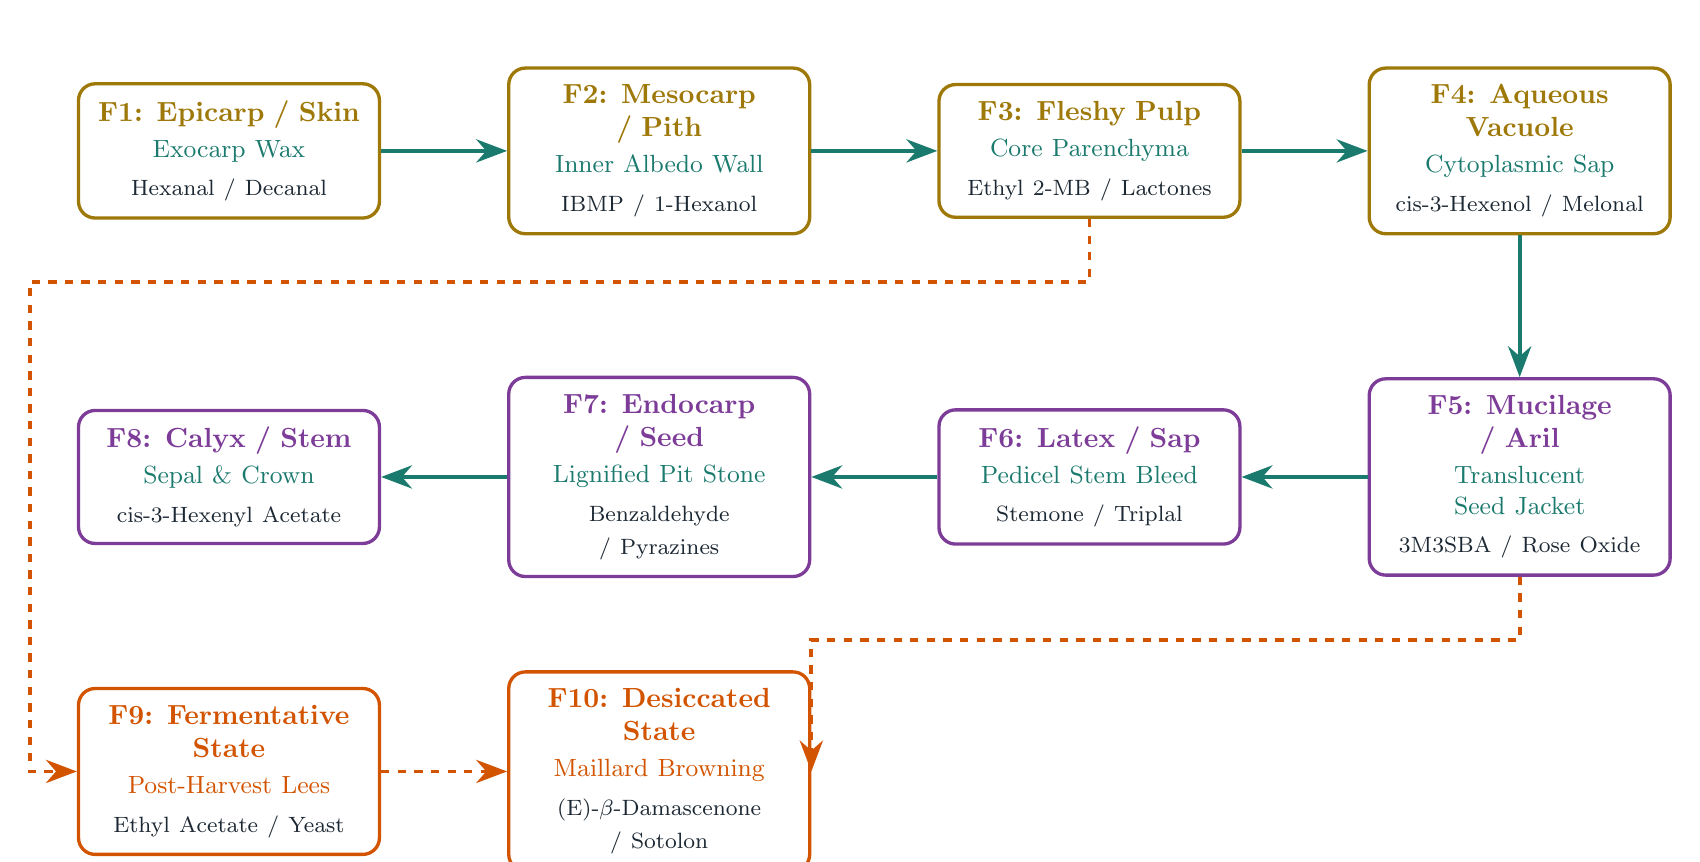
\begin{tikzpicture}[
    node distance=1.4cm and 1.6cm,
    facetgold/.style={draw=GoldDark, fill=white, rounded corners=6pt, line width=1.2pt, inner sep=6pt, text width=3.4cm, align=center, execute at begin node={\hyphenpenalty=10000 \exhyphenpenalty=10000}},
    facetpurple/.style={draw=PurpleAccent, fill=white, rounded corners=6pt, line width=1.2pt, inner sep=6pt, text width=3.4cm, align=center, execute at begin node={\hyphenpenalty=10000 \exhyphenpenalty=10000}},
    facetrust/.style={draw=RustAccent, fill=white, rounded corners=6pt, line width=1.2pt, inner sep=6pt, text width=3.4cm, align=center, execute at begin node={\hyphenpenalty=10000 \exhyphenpenalty=10000}},
    arrow/.style={-{Stealth[scale=1.2]}, line width=1.4pt, draw=TealAccent},
    decayarrow/.style={-{Stealth[scale=1.2]}, line width=1.4pt, draw=RustAccent, dashed}
]

% Spatial Layer Nodes (Row 1)
\node[facetgold] (F1) {{\bfseries\color{GoldDark} F1: Epicarp / Skin}\\[2pt] \small\color{TealAccent} Exocarp Wax\\[2pt] \footnotesize\color{TextDark} Hexanal / Decanal};
\node[facetgold, right=of F1] (F2) {{\bfseries\color{GoldDark} F2: Mesocarp / Pith}\\[2pt] \small\color{TealAccent} Inner Albedo Wall\\[2pt] \footnotesize\color{TextDark} IBMP / 1-Hexanol};
\node[facetgold, right=of F2] (F3) {{\bfseries\color{GoldDark} F3: Fleshy Pulp}\\[2pt] \small\color{TealAccent} Core Parenchyma\\[2pt] \footnotesize\color{TextDark} Ethyl 2-MB / Lactones};
\node[facetgold, right=of F3] (F4) {{\bfseries\color{GoldDark} F4: Aqueous Vacuole}\\[2pt] \small\color{TealAccent} Cytoplasmic Sap\\[2pt] \footnotesize\color{TextDark} cis-3-Hexenol / Melonal};

% Anatomical Seed & Stem Nodes (Row 2, placed cleanly under Row 1)
\node[facetpurple, below=1.8cm of F4] (F5) {{\bfseries\color{PurpleAccent} F5: Mucilage / Aril}\\[2pt] \small\color{TealAccent} Translucent Seed Jacket\\[2pt] \footnotesize\color{TextDark} 3M3SBA / Rose Oxide};
\node[facetpurple, left=of F5] (F6) {{\bfseries\color{PurpleAccent} F6: Latex / Sap}\\[2pt] \small\color{TealAccent} Pedicel Stem Bleed\\[2pt] \footnotesize\color{TextDark} Stemone / Triplal};
\node[facetpurple, left=of F6] (F7) {{\bfseries\color{PurpleAccent} F7: Endocarp / Seed}\\[2pt] \small\color{TealAccent} Lignified Pit Stone\\[2pt] \footnotesize\color{TextDark} Benzaldehyde / Pyrazines};
\node[facetpurple, left=of F7] (F8) {{\bfseries\color{PurpleAccent} F8: Calyx / Stem}\\[2pt] \small\color{TealAccent} Sepal \& Crown\\[2pt] \footnotesize\color{TextDark} cis-3-Hexenyl Acetate};

% Thermal Transformation Nodes (Row 3, placed cleanly below F8 & F7)
\node[facetrust, below=1.8cm of F8] (F9) {{\bfseries\color{RustAccent} F9: Fermentative State}\\[2pt] \small\color{RustAccent} Post-Harvest Lees\\[2pt] \footnotesize\color{TextDark} Ethyl Acetate / Yeast};
\node[facetrust, right=of F9] (F10) {{\bfseries\color{RustAccent} F10: Desiccated State}\\[2pt] \small\color{RustAccent} Maillard Browning\\[2pt] \footnotesize\color{TextDark} (E)-$\beta$-Damascenone / Sotolon};

% Spatial Sequential Flow (Solid Teal Arrows)
\draw[arrow] (F1) -- (F2);
\draw[arrow] (F2) -- (F3);
\draw[arrow] (F3) -- (F4);
\draw[arrow] (F4) -- (F5);
\draw[arrow] (F5) -- (F6);
\draw[arrow] (F6) -- (F7);
\draw[arrow] (F7) -- (F8);

% 100% Non-Overlapping Decay Routing
\draw[decayarrow] (F3.south) -- ++(0,-0.8) -| ($(F8.west)+(-0.6,0)$) |- (F9.west);
\draw[decayarrow] (F5.south) -- ++(0,-0.8) -| (F10.east);
\draw[decayarrow] (F9.east) -- (F10.west);

\end{tikzpicture}%
}
\caption{Topological lifecycle flow map of the 10 fruit facets showing non-overlapping spatial tissue sequencing and thermal post-harvest decay.}
\label{fig:lifecycle}
\end{figure}

\vspace{1em}

% ==========================================
% FIGURE 2: FACET RATIO DONUT FINGERPRINTS
% ==========================================
\begin{figure}[htbp]
\centering
\resizebox{\textwidth}{!}{%
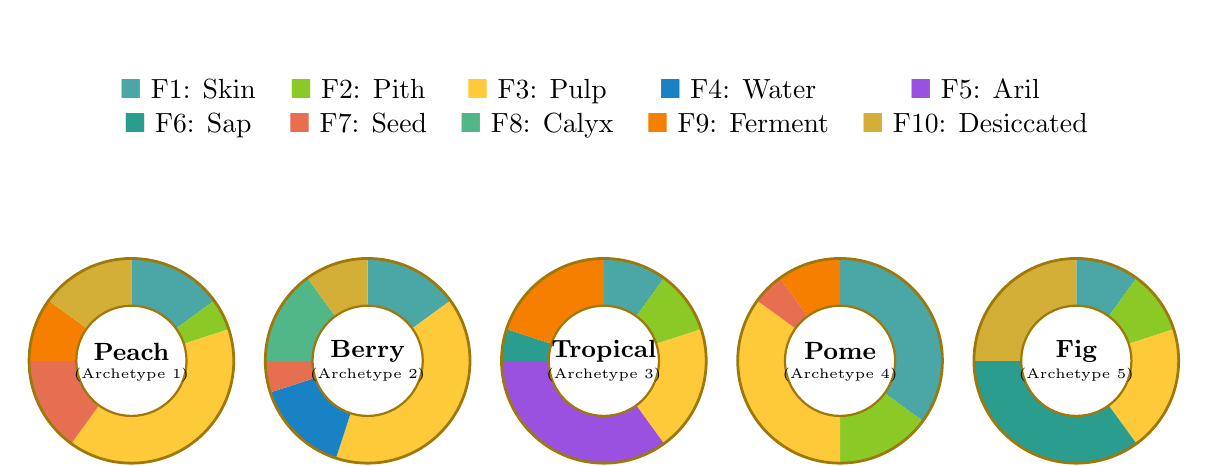
\begin{tikzpicture}

% --- LEGEND BAR (TOP) ---
\node at (0, 3.2) [anchor=center] {%
  \begin{tabular}{ccccc}
    \textcolor{pF1}{$\blacksquare$} F1: Skin & \textcolor{pF2}{$\blacksquare$} F2: Pith & \textcolor{pF3}{$\blacksquare$} F3: Pulp & \textcolor{pF4}{$\blacksquare$} F4: Water & \textcolor{pF5}{$\blacksquare$} F5: Aril \\
    \textcolor{pF6}{$\blacksquare$} F6: Sap & \textcolor{pF7}{$\blacksquare$} F7: Seed & \textcolor{pF8}{$\blacksquare$} F8: Calyx & \textcolor{pF9}{$\blacksquare$} F9: Ferment & \textcolor{pF10}{$\blacksquare$} F10: Desiccated
  \end{tabular}
};

% --- DONUT 1: PEACH (Stone Fruit Archetype 1) ---
\begin{scope}[shift={(-6,0)}]
    % Slices
    \fill[pF1] (0,0) -- (90:1.3) arc (90:36:1.3) -- cycle;    % 15%
    \fill[pF2] (0,0) -- (36:1.3) arc (36:18:1.3) -- cycle;    % 5%
    \fill[pF3] (0,0) -- (18:1.3) arc (18:-126:1.3) -- cycle;  % 40%
    \fill[pF7] (0,0) -- (-126:1.3) arc (-126:-180:1.3) -- cycle; % 15%
    \fill[pF9] (0,0) -- (-180:1.3) arc (-180:-216:1.3) -- cycle; % 10%
    \fill[pF10] (0,0) -- (-216:1.3) arc (-216:-270:1.3) -- cycle; % 15%
    % Center Hole
    \fill[white] (0,0) circle (0.7);
    \draw[line width=1pt, GoldDark] (0,0) circle (1.3);
    \draw[line width=0.8pt, GoldDark] (0,0) circle (0.7);
    \node at (0,0.12) {\bfseries\small Peach};
    \node at (0,-0.18) {\tiny (Archetype 1)};
\end{scope}

% --- DONUT 2: STRAWBERRY (Red Berries Archetype 2) ---
\begin{scope}[shift={(-3,0)}]
    \fill[pF1] (0,0) -- (90:1.3) arc (90:36:1.3) -- cycle;    % 15%
    \fill[pF3] (0,0) -- (36:1.3) arc (36:-108:1.3) -- cycle;  % 40%
    \fill[pF4] (0,0) -- (-108:1.3) arc (-108:-162:1.3) -- cycle; % 15%
    \fill[pF7] (0,0) -- (-162:1.3) arc (-162:-180:1.3) -- cycle; % 5%
    \fill[pF8] (0,0) -- (-180:1.3) arc (-180:-234:1.3) -- cycle; % 15%
    \fill[pF10] (0,0) -- (-234:1.3) arc (-234:-270:1.3) -- cycle; % 10%
    \fill[white] (0,0) circle (0.7);
    \draw[line width=1pt, GoldDark] (0,0) circle (1.3);
    \draw[line width=0.8pt, GoldDark] (0,0) circle (0.7);
    \node at (0,0.12) {\bfseries\small Berry};
    \node at (0,-0.18) {\tiny (Archetype 2)};
\end{scope}

% --- DONUT 3: PASSIONFRUIT (Tropical Archetype 3) ---
\begin{scope}[shift={(0,0)}]
    \fill[pF1] (0,0) -- (90:1.3) arc (90:54:1.3) -- cycle;    % 10%
    \fill[pF2] (0,0) -- (54:1.3) arc (54:18:1.3) -- cycle;    % 10%
    \fill[pF3] (0,0) -- (18:1.3) arc (18:-54:1.3) -- cycle;   % 20%
    \fill[pF5] (0,0) -- (-54:1.3) arc (-54:-180:1.3) -- cycle; % 35%
    \fill[pF6] (0,0) -- (-180:1.3) arc (-180:-198:1.3) -- cycle; % 5%
    \fill[pF9] (0,0) -- (-198:1.3) arc (-198:-270:1.3) -- cycle; % 20%
    \fill[white] (0,0) circle (0.7);
    \draw[line width=1pt, GoldDark] (0,0) circle (1.3);
    \draw[line width=0.8pt, GoldDark] (0,0) circle (0.7);
    \node at (0,0.12) {\bfseries\small Tropical};
    \node at (0,-0.18) {\tiny (Archetype 3)};
\end{scope}

% --- DONUT 4: GREEN APPLE (Pome Archetype 4) ---
\begin{scope}[shift={(3,0)}]
    \fill[pF1] (0,0) -- (90:1.3) arc (90:-36:1.3) -- cycle;   % 35%
    \fill[pF2] (0,0) -- (-36:1.3) arc (-36:-90:1.3) -- cycle; % 15%
    \fill[pF3] (0,0) -- (-90:1.3) arc (-90:-216:1.3) -- cycle; % 35%
    \fill[pF7] (0,0) -- (-216:1.3) arc (-216:-234:1.3) -- cycle; % 5%
    \fill[pF9] (0,0) -- (-234:1.3) arc (-234:-270:1.3) -- cycle; % 10%
    \fill[white] (0,0) circle (0.7);
    \draw[line width=1pt, GoldDark] (0,0) circle (1.3);
    \draw[line width=0.8pt, GoldDark] (0,0) circle (0.7);
    \node at (0,0.12) {\bfseries\small Pome};
    \node at (0,-0.18) {\tiny (Archetype 4)};
\end{scope}

% --- DONUT 5: FIG ILLUSION (Green/Woody Archetype 5) ---
\begin{scope}[shift={(6,0)}]
    \fill[pF1] (0,0) -- (90:1.3) arc (90:54:1.3) -- cycle;    % 10%
    \fill[pF2] (0,0) -- (54:1.3) arc (54:18:1.3) -- cycle;    % 10%
    \fill[pF3] (0,0) -- (18:1.3) arc (18:-54:1.3) -- cycle;   % 20%
    \fill[pF6] (0,0) -- (-54:1.3) arc (-54:-180:1.3) -- cycle; % 35%
    \fill[pF10] (0,0) -- (-180:1.3) arc (-180:-270:1.3) -- cycle; % 25%
    \fill[white] (0,0) circle (0.7);
    \draw[line width=1pt, GoldDark] (0,0) circle (1.3);
    \draw[line width=0.8pt, GoldDark] (0,0) circle (0.7);
    \node at (0,0.12) {\bfseries\small Fig};
    \node at (0,-0.18) {\tiny (Archetype 5)};
\end{scope}

\end{tikzpicture}%
}
\caption{Facet Olfactory Ratio Donut Charts (Visual Color Fingerprints) showing 3D anatomical volume distribution across representative Fruit Archetype families.}
\label{fig:donuts}
\end{figure}

\newpage

% ==========================================
% SECTION 3: EXHAUSTIVE 10-FACET DEEP DIVE
% ==========================================
\section{Exhaustive Anatomical Facet Specifications}

\subsection{Facet 1: Epicarp / Skin (Outer Exocarp \& Flavedo Wax)}

\begin{botanicalbox}
\textbf{Origin:} Outer Exocarp \& Citrus Flavedo Wax Layer.\\
\textbf{Anatomical Function:} The protective outer skin envelope containing hydrophobic plant waxes, alicyclic terpenes, green leaf aldehydes ($C_6$), and aliphatic citrus flavedo aldehydes ($C_8, C_{10}$).
\end{botanicalbox}

\begin{sensoryquote}
"The physical sensation of biting into a taut green apple peel or scratching a fresh orange rind---driven by green leaf aldehydes ($C_6$), waxy citrus flavedo aldehydes ($C_8/C_{10}$ Decanal), and peppery skin terpenes (Myrcene, Limonene)."
\end{sensoryquote}

\begin{flavourbox}
\textbf{Tactile \& Palate Experience:} Biting green skin friction, snappy exocarp resistance on teeth, and zesty, peppery essential oil warmth on the lips. Provides necessary structural astringency to cut through heavy fruit sugars.
\end{flavourbox}

\begin{table}[htbp]
\centering
\caption{Primary Impact Actors for Facet 1 (Epicarp / Skin)}
\vspace{0.3em}
\resizebox{\textwidth}{!}{%
\begin{tabular}{lcccccc}
\toprule
\textbf{Compound Name} & \textbf{CAS No.} & \textbf{SMILES} & \textbf{MW} & \textbf{VP (Pa)} & \textbf{Threshold} & \textbf{Primary Role} \\
\midrule
Hexanal & 66-25-1 & \texttt{CCCCCC=O} & 100.16 & 1,500.0 & 500.0 ppb & Crisp $C_6$ green apple skin aldehyde \\
(E)-2-Hexenal & 6728-26-3 & \texttt{CCC/C=C/C=O} & 98.14 & 480.0 & 17.0 ppb & Taut green peel \& leaf bite (\texttt{4GA02582}) \\
Decanal ($C_{10}$) & 112-31-2 & \texttt{CCCCCCCCCC=O} & 156.27 & 25.0 & 0.1 ppb & Pungent citrus flavedo wax \& orange rind \\
d-Limonene & 5989-27-5 & \texttt{CC1=CCC(CC1)C(=C)C} & 136.23 & 190.0 & 200.0 ppb & Citrus peel terpene hydrocarbon \\
\bottomrule
\end{tabular}%
}
\end{table}

\textbf{Modifiers \& Fixatives:} Octanal ($C_8$), Sinensal, Myrcene | \textbf{Fixatives:} Cold-Pressed Citrus Oils, Linalyl Acetate.

\vspace{1.5em}

\subsection{Facet 2: Mesocarp / Pith (Inner Albedo \& Cellulosic Parenchyma)}

\begin{botanicalbox}
\textbf{Origin:} Inner Albedo Wall \& Cellulosic Parenchyma.\\
\textbf{Anatomical Function:} The spongy, un-pigmented white layer beneath citrus exocarp or melon inner rind. Provides dry, cellulosic, bitter green friction that prevents fruit formulas from collapsing into synthetic candy.
\end{botanicalbox}

\begin{sensoryquote}
"The astringent, dry inner white pith of a grapefruit or rhubarb stalk. Prevents synthetic ester sweetness from feeling flat."
\end{sensoryquote}

\begin{flavourbox}
\textbf{Tactile \& Palate Experience:} Spongy, mouth-drying cellulosic texture. Delivers bitter albedo astringency on the back sides of the tongue, grounding diffusive top-note sweetness.
\end{flavourbox}

\begin{table}[htbp]
\centering
\caption{Primary Impact Actors for Facet 2 (Mesocarp / Pith)}
\vspace{0.3em}
\resizebox{\textwidth}{!}{%
\begin{tabular}{lcccccc}
\toprule
\textbf{Compound Name} & \textbf{CAS No.} & \textbf{SMILES} & \textbf{MW} & \textbf{VP (Pa)} & \textbf{Threshold} & \textbf{Primary Role} \\
\midrule
Isobutyl Methoxypyrazine & 24683-00-9 & \texttt{CC(C)CC1=CN=C(C=N1)OC} & 166.22 & 12.0 & 0.002 ppb & Pith pyrazine (ultra-potent) \\
1-Hexanol & 111-27-3 & \texttt{CCCCCC[OH]} & 102.17 & 124.0 & 500.0 ppb & Oily cellulosic alcohol \\
2-Isopropyl-4-methylthiazole & 15679-13-7 & \texttt{CC(C)C1=NC=C(C)S1} & 141.23 & 15.0 & 3.0 ppb & Bitter green albedo thiazole \\
\bottomrule
\end{tabular}%
}
\end{table}

\textbf{Modifiers \& Fixatives:} Stemone, Rhubofix | \textbf{Fixatives:} Veramoss (Evernyl), Cedrol (Cedarwood), Cashmeran.

\newpage

\subsection{Facet 3: Fleshy Pulp (Core Parenchyma \& Aril Juice Cells)}

\begin{botanicalbox}
\textbf{Origin:} Core Parenchyma \& Ripe Juice Sacs.\\
\textbf{Anatomical Function:} The dominant sweet core identity of the fruit, rich in aliphatic esters, short-chain lactones, and fruit acids.
\end{botanicalbox}

\begin{sensoryquote}
"Biting into the sweet, dripping heart of a perfectly ripe peach or passionfruit."
\end{sensoryquote}

\begin{flavourbox}
\textbf{Tactile \& Palate Experience:} Succulent, dripping sweetness, lush fruit nectar coating the mid-palate, and velvety peach/apricot mouthfeel driven by short-chain gamma-lactones.
\end{flavourbox}

\begin{table}[htbp]
\centering
\caption{Primary Impact Actors for Facet 3 (Fleshy Pulp)}
\vspace{0.3em}
\resizebox{\textwidth}{!}{%
\begin{tabular}{lcccccc}
\toprule
\textbf{Compound Name} & \textbf{CAS No.} & \textbf{SMILES} & \textbf{MW} & \textbf{VP (Pa)} & \textbf{Threshold} & \textbf{Primary Role} \\
\midrule
Ethyl Butanoate & 105-54-4 & \texttt{CCCC(=O)OCC} & 116.16 & 1,700.0 & 1.0 ppb & Diffusive juicy top ester \\
Ethyl 2-Methylbutanoate & 7452-79-1 & \texttt{CCC(C)C(=O)OCC} & 130.18 & 320.0 & 0.01 ppb & Ripe pulp driver \\
Ethyl Hexanoate & 123-66-0 & \texttt{CCCCCC(=O)OCC} & 144.21 & 210.0 & 1.0 ppb & Juicy pineapple/apple flesh \\
$\gamma$-Decalactone & 706-14-9 & \texttt{CCCCCCC1CCC(=O)O1} & 170.25 & 0.12 & 100.0 ppb & Velvety peach flesh lactone \\
\bottomrule
\end{tabular}%
}
\end{table}

\textbf{Modifiers \& Fixatives:} Allyl Caproate, Pear Ester, Methyl Benzoate | \textbf{Fixatives:} Hedione, Habanolide / Helvetolide.

\vspace{1.5em}

\subsection{Facet 4: Aqueous Vacuole (Cytoplasmic Sap \& Cellular Water)}

\begin{botanicalbox}
\textbf{Origin:} Cytoplasmic Water \& Vacuole Nectar Sap.\\
\textbf{Anatomical Function:} High-moisture cellular water that bursts during slicing, creating a dewy spray cloud.
\end{botanicalbox}

\begin{sensoryquote}
"The humid, cool spray cloud that bursts into the air when slicing open a fresh melon or cucumber."
\end{sensoryquote}

\begin{flavourbox}
\textbf{Tactile \& Palate Experience:} Ice-cold watery hydration, a cooling mist on the palate, and aquatic cucumber/melon freshness that lifts heavy fruit pulp into airy sillage.
\end{flavourbox}

\begin{table}[htbp]
\centering
\caption{Primary Impact Actors for Facet 4 (Aqueous Vacuole)}
\vspace{0.3em}
\resizebox{\textwidth}{!}{%
\begin{tabular}{lcccccc}
\toprule
\textbf{Compound Name} & \textbf{CAS No.} & \textbf{SMILES} & \textbf{MW} & \textbf{VP (Pa)} & \textbf{Threshold} & \textbf{Primary Role} \\
\midrule
cis-3-Hexenol & 928-96-1 & \texttt{CCC=CCCO} & 100.16 & 200.0 & 70.0 ppb & Fresh green dew alcohol \\
Melonal & 106-72-9 & \texttt{CC(C)=CCCC(C)C=O} & 142.24 & 140.0 & 0.5 ppb & Watery melon juice aldehyde \\
(2E,6Z)-Nonadienal & 557-48-2 & \texttt{CCC=CCC=CCC=O} & 138.21 & 22.0 & 0.01 ppb & Aqueous cucumber sap aldehyde \\
Calone 1951 & 28940-11-6 & \texttt{CC1=CC2=C(C=C1)OCC(=O)CO2} & 178.18 & 0.05 & 0.03 ppb & Marine-watery humidity \\
\bottomrule
\end{tabular}%
}
\end{table}

\textbf{Modifiers \& Fixatives:} Hydroxycitronellal, Bourgeonal, Cyclamen Aldehyde, Floralozone, Vernaldehyde | \textbf{Fixatives:} Helional, Florhydral.

\newpage

\subsection{Facet 5: Mucilage / Aril (Translucent Seed Jacket)}

\begin{botanicalbox}
\textbf{Origin:} Translucent Seed Jacket \& Aril Envelope (Lychee, Pomegranate, Mangosteen).\\
\textbf{Anatomical Function:} Gelatinous, slippery seed jackets rich in volatile thiols, rose ketones, and delta-lactones.
\end{botanicalbox}

\begin{sensoryquote}
"The slippery, pearlescent mucilage jacket surrounding pomegranate, lychee, or mangosteen seeds---delivering translucent fruit nectar with a trace tropical sulfur spark."
\end{sensoryquote}

\begin{flavourbox}
\textbf{Tactile \& Palate Experience:} Slippery, pearlescent mucilage coating the mouth. Delivers a combination of sparkling floral-lychee sweetness and an electrifying, exotic tropical sulfur bite.
\end{flavourbox}

\begin{table}[htbp]
\centering
\caption{Primary Impact Actors for Facet 5 (Mucilage / Aril)}
\vspace{0.3em}
\resizebox{\textwidth}{!}{%
\begin{tabular}{lcccccc}
\toprule
\textbf{Compound Name} & \textbf{CAS No.} & \textbf{SMILES} & \textbf{MW} & \textbf{VP (Pa)} & \textbf{Threshold} & \textbf{Primary Role} \\
\midrule
3M3SBA & 5287-43-4 & \texttt{CC(=O)OCCC(C)(C)S} & 162.25 & 18.0 & 0.05 ppb & Mangosteen \& durian aril thiol \\
$\delta$-Decalactone & 705-86-2 & \texttt{CCCCCC1CCCC(=O)O1} & 170.25 & 0.08 & 100.0 ppb & Creamy lactone seed jacket membrane \\
cis-Rose Oxide & 4889-45-7 & \texttt{CC1CCC(O1)C=C(C)C} & 154.25 & 110.0 & 0.5 ppb & Sparkling lychee \& pomegranate bloom \\
\bottomrule
\end{tabular}%
}
\end{table}

\textbf{Modifiers \& Fixatives:} 3MH (3-Mercaptohexanol), Ethyl Lactate, Veloutone | \textbf{Fixatives:} Ethylene Brassylate, $\gamma$-Nonalactone (C18), Hydroxycitronellal.

\vspace{1.5em}

\subsection{Facet 6: Latex / Sap (Pedicel Stem Bleed \& Shrub Resin)}

\begin{botanicalbox}
\textbf{Origin:} Pedicel Stem Bleed \& Shrub Resin Ducts.\\
\textbf{Anatomical Function:} Milky, rubbery stem sap containing oximes and cyclo-aliphatic aldehydes.
\end{botanicalbox}

\begin{sensoryquote}
"The milky, bitter, raw sap that bleeds when snapping a green fig stem or unpeeling raw papaya."
\end{sensoryquote}

\begin{flavourbox}
\textbf{Tactile \& Palate Experience:} Sticky, rubbery latex residue on fingers. Biting green sap bitterness and a milky-vegetal resinous film that lingers on the back of the tongue.
\end{flavourbox}

\begin{table}[htbp]
\centering
\caption{Primary Impact Actors for Facet 6 (Latex / Sap)}
\vspace{0.3em}
\resizebox{\textwidth}{!}{%
\begin{tabular}{lcccccc}
\toprule
\textbf{Compound Name} & \textbf{CAS No.} & \textbf{SMILES} & \textbf{MW} & \textbf{VP (Pa)} & \textbf{Threshold} & \textbf{Primary Role} \\
\midrule
Stemone & 22457-23-4 & \texttt{CCC(C)CC(=NO)CC} & 141.21 & 28.0 & 10.0 ppb & Fig leaf milk \& papaya sap oxime \\
Triplal / Isocyclocitral & 68039-49-6 & \texttt{CC1=CCC(C)C(C=O)C1} & 138.21 & 90.0 & 0.5 ppb & Raw snapped stem sap aldehyde \\
\bottomrule
\end{tabular}%
}
\end{table}

\textbf{Modifiers \& Fixatives:} cis-3-Hexenyl Salicylate, Allyl Amyl Glycolate | \textbf{Fixatives:} Vertofix Coeur, Iso E Super.

\newpage

\subsection{Facet 7: Endocarp / Seed (Lignified Pit Stone \& Kernel Oil)}

\begin{botanicalbox}
\textbf{Origin:} Lignified Seed Core, Pit Stone \& Kernel Oil.\\
\textbf{Anatomical Function:} Lignified seed stone containing cyanic nitriles, aromatic aldehydes, and roasted pyrazines.
\end{botanicalbox}

\begin{sensoryquote}
"The rich, cyanic, woody bitterness inside a cracked cherry pit or peach stone."
\end{sensoryquote}

\begin{flavourbox}
\textbf{Tactile \& Palate Experience:} Hard wooden shell texture, intense cyanic amaretto/marzipan bitterness, and roasted nutty oiliness in the retronasal passage.
\end{flavourbox}

\begin{table}[htbp]
\centering
\caption{Primary Impact Actors for Facet 7 (Endocarp / Seed)}
\vspace{0.3em}
\resizebox{\textwidth}{!}{%
\begin{tabular}{lcccccc}
\toprule
\textbf{Compound Name} & \textbf{CAS No.} & \textbf{SMILES} & \textbf{MW} & \textbf{VP (Pa)} & \textbf{Threshold} & \textbf{Primary Role} \\
\midrule
Benzaldehyde & 100-52-7 & \texttt{O=Cc1ccccc1} & 106.12 & 127.0 & 350.0 ppb & Cyanic cherry/peach pit core \\
2,3,5-Trimethylpyrazine & 14667-55-1 & \texttt{Cc1cnc(C)c(C)n1} & 122.17 & 110.0 & 1,000.0 ppb & Roasted nutty seed pyrazine \\
2-Acetylpyrazine & 22047-25-2 & \texttt{CC(=O)c1cnccn1} & 122.13 & 145.0 & 60.0 ppb & Toasted seed core pyrazine \\
\bottomrule
\end{tabular}%
}
\end{table}

\textbf{Modifiers \& Fixatives:} Heliotropin (Piperonal), Cinnamyl Acetate, Eugenol | \textbf{Fixatives:} Coumarin, Vanillin, Benzoin Resinoid.

\vspace{1.5em}

\subsection{Facet 8: Calyx / Stem (Leaf Sepals \& Peduncle Crown)}

\begin{botanicalbox}
\textbf{Origin:} Leaf Sepals \& Peduncle Crown Base.\\
\textbf{Anatomical Function:} Leafy green sepal crown attached to fruit tops (strawberry, tomato, cherry).
\end{botanicalbox}

\begin{sensoryquote}
"The crisp, tart, raw greenness of sepal leaves attached to the top of a strawberry or cherry peduncle."
\end{sensoryquote}

\begin{flavourbox}
\textbf{Tactile \& Palate Experience:} Crisp leaf crown snap, biting garden leaf acidity, and tart rhubarb sepal astringency on the sides of the palate.
\end{flavourbox}

\begin{table}[htbp]
\centering
\caption{Primary Impact Actors for Facet 8 (Calyx / Stem)}
\vspace{0.3em}
\resizebox{\textwidth}{!}{%
\begin{tabular}{lcccccc}
\toprule
\textbf{Compound Name} & \textbf{CAS No.} & \textbf{SMILES} & \textbf{MW} & \textbf{VP (Pa)} & \textbf{Threshold} & \textbf{Primary Role} \\
\midrule
cis-3-Hexenyl Acetate & 3681-71-8 & \texttt{CCC=CCCOC(=O)C} & 142.20 & 180.0 & 25.0 ppb & Fresh leaf crown \& green top \\
Styralyl Acetate & 93-92-5 & \texttt{CC(OC(=O)C)c1ccccc1} & 164.20 & 20.0 & 1.2 ppb & Tart rhubarb calyx bite \\
\bottomrule
\end{tabular}%
}
\end{table}

\textbf{Modifiers \& Fixatives:} Hexyl Acetate, cis-3-Hexenyl Isobutyrate | \textbf{Fixatives:} Diphenyl Oxide, Geranyl Acetate.

\newpage

\subsection{Facet 9: Fermentative State (Post-Harvest Glycolysis \& Yeast Lees)}

\begin{botanicalbox}
\textbf{Origin:} Post-Harvest Glycolysis \& Overripe Lees Transformation.\\
\textbf{Anatomical Function:} Fermentative transformation producing boozy esters, volatile acetic acid, and yeast fusel alcohols.
\end{botanicalbox}

\begin{sensoryquote}
"The intoxicating, rummy, warm alcoholic sparkle of fermenting plum lees or vintage cider."
\end{sensoryquote}

\begin{flavourbox}
\textbf{Tactile \& Palate Experience:} Volatile alcoholic warmth in the throat, rummy yeast lees richness, and a tangy fermented fruit cider sparkle.
\end{flavourbox}

\begin{table}[htbp]
\centering
\caption{Primary Impact Actors for Facet 9 (Fermentative State)}
\vspace{0.3em}
\resizebox{\textwidth}{!}{%
\begin{tabular}{lcccccc}
\toprule
\textbf{Compound Name} & \textbf{CAS No.} & \textbf{SMILES} & \textbf{MW} & \textbf{VP (Pa)} & \textbf{Threshold} & \textbf{Primary Role} \\
\midrule
Ethyl Acetate & 141-78-6 & \texttt{CC(=O)OCC} & 88.11 & 9,700.0 & 5,000.0 ppb & Volatile boozy lift ester \\
Isoamyl Acetate & 123-92-2 & \texttt{CC(=O)OCCC(C)C} & 130.18 & 530.0 & 2.0 ppb & Rummy banana yeast ester \\
\bottomrule
\end{tabular}%
}
\end{table}

\textbf{Modifiers \& Fixatives:} Isovaleric Acid | \textbf{Fixatives:} Green Cognac Oil, PEA (Phenylethyl Alcohol).

\vspace{1.5em}

\subsection{Facet 10: Desiccated State (Maillard Browning \& Dehydrated Fruit Paste)}

\begin{botanicalbox}
\textbf{Origin:} Non-Enzymatic Maillard Browning \& Fruit Dehydration.\\
\textbf{Anatomical Function:} Thermal sugar-amino acid caramelization occurring in dried persimmons (Hoshigaki), dates, prunes, and cooked jams.
\end{botanicalbox}

\begin{sensoryquote}
"Rich, dark, sticky preserve paste, sun-dried persimmons (Hoshigaki), Medjool dates, dried Agen prunes, and caramelized fruit preserves."
\end{sensoryquote}

\begin{flavourbox}
\textbf{Tactile \& Palate Experience:} Dense, sticky, chewy fruit paste mouthfeel. Rich caramelized fructose, fenugreek/molasses warmth, and lingering sun-baked persimmon richness.
\end{flavourbox}

\begin{table}[htbp]
\centering
\caption{Primary Impact Actors for Facet 10 (Desiccated State)}
\vspace{0.3em}
\resizebox{\textwidth}{!}{%
\begin{tabular}{lcccccc}
\toprule
\textbf{Compound Name} & \textbf{CAS No.} & \textbf{SMILES} & \textbf{MW} & \textbf{VP (Pa)} & \textbf{Threshold} & \textbf{Primary Role} \\
\midrule
(E)-$\beta$-Damascenone & 23696-85-7 & \texttt{CC(=O)/C=C/C1=C(C)C=CCC1(C)C} & 190.28 & 0.25 & 0.002 ppb & Cooked plum driver (ppt) \\
Furaneol (DMHF) & 3658-77-3 & \texttt{CC1=C(C(=O)C(O1)C)O} & 128.13 & 0.08 & 0.05 ppb & Burnt sugar \& strawberry paste \\
Sotolon & 28588-74-1 & \texttt{CC1C(=C(C(=O)O1)O)C} & 128.13 & 0.02 & 0.001 ppb & Caramelized fenugreek \& fig \\
$\beta$-Ionone & 14901-07-6 & \texttt{CC1=C(/C=C/C(=O)C)C(C)(C)CCC1} & 192.30 & 0.96 & 0.007 ppb & Sun-dried fruit paste driver \\
\bottomrule
\end{tabular}%
}
\end{table}

\textbf{Modifiers \& Fixatives:} Ethyl Maltol, Maltol | \textbf{Fixatives:} Ethyl Vanillin, Coumarin, Benzoin Resinoid.

\newpage

% ==========================================
% SECTION 4: LANDSCAPE MASTER 10x10 MATRIX
% ==========================================
\begin{landscape}
\section{The Master \texorpdfstring{10$\times$10}{10x10} Fruit Archetype Matrix}

Table \ref{tab:matrix_full} provides the comprehensive 100-cell chemical mapping across all 10 Fruit Archetypes and 10 Facets of the Anatomical Lifecycle Engine.

\begin{table}[htbp]
\centering
\caption{Master \texorpdfstring{10$\times$10}{10x10} Fruit Archetype Matrix (Exhaustive 100-Cell Primary Chemical Mapping)}
\label{tab:matrix_full}
\vspace{0.5em}
\resizebox{\linewidth}{!}{%
\begin{tabular}{l cccccccccc}
\toprule
\textbf{Archetype} & \textbf{F1: Skin} & \textbf{F2: Pith} & \textbf{F3: Pulp} & \textbf{F4: Vacuole} & \textbf{F5: Aril} & \textbf{F6: Sap} & \textbf{F7: Seed} & \textbf{F8: Calyx} & \textbf{F9: Ferment} & \textbf{F10: Desiccated} \\
\midrule
\textbf{1. Apple} & Hexanal & 1-Hexanol & Ethyl 2-MB & cis-3-Hexenol & Hexyl Butanoate & Triplal & Benzaldehyde & cis-3-Hexenyl Acetate & Ethyl Acetate & Damascenone \\
\textbf{2. Citrus} & Decanal C10 & Octanal & Limonene & Melonal & Nootkatone & Stemone & Limonin & Linalyl Acetate & Ethyl Butanoate & Citral \\
\textbf{3. Peach} & (E)-2-Hexenal & Velvione & $\gamma$-Decalactone & cis-3-Hexenol & $\delta$-Decalactone & Stemone & Benzaldehyde & Styralyl Acetate & Ethyl Acetate & Sotolon \\
\textbf{4. Strawberry} & Hexyl Acetate & Methyl Cinnamate & Furaneol & Melonal & Aldehyde C16 & cis-3-Hexenyl Benzoate & Diethyl Methylpyrazine & cis-3-Hexenyl Acetate & Ethyl Isobutyrate & DMHF \\
\textbf{5. Mango} & Myrcene & Ocimene & Ethyl Hexanoate & Melonal & 3M3SBA & Terpinolene & Guaiacol & Delta-3-Carene & Isoamyl Acetate & Sotolon \\
\textbf{6. Passionfruit} & Oxane & 1-Hexanol & Ethyl Butanoate & Melonal & 3M3SBA & Stemone & Caryophyllene & Linalool & Ethyl Acetate & Damascenone \\
\textbf{7. Grape} & Myrcene & Methyl Anthranilate & Ethyl Isovalerate & Nonadienal & cis-Rose Oxide & cis-3-Hexenyl Acetate & Tannin & Ethyl Safranate & Ethyl Acetate & Furaneol \\
\textbf{8. Cherry} & Benzaldehyde & Ionone Alpha & Benzyl Acetate & Anisaldehyde & cis-Rose Oxide & Benzoin Resinoid & Benzaldehyde & Styralyl Acetate & Isoamyl Alcohol & Damascenone \\
\textbf{9. Fig} & $\gamma$-Octalactone & IBMP & $\gamma$-Decalactone & cis-3-Hexenol & Oxyphenylon & Stemone & Pyrazines & cis-3-Hexenyl Salicylate & Ethyl Butanoate & Sotolon \\
\textbf{10. Pineapple} & Allyl Cyclohexylprop. & Ethyl 3-Methylthioprop. & Allyl Hexanoate & Melonal & Fructone & AAG & Phenethyl Isobutyrate & AAG & Ethyl Acetate & DMHF \\
\bottomrule
\end{tabular}%
}
\end{table}

\end{landscape}

\newpage

% ==========================================
% SECTION 5: FORMULATION SOP
% ==========================================
\section{Formulation Standard Operating Procedure (SOP)}

To compounding living fruit accords without ester collapse, follow these three golden formulation protocols:

\subsection{1. Ultra-Low Threshold Dosing Rules}
High-potency impact chemicals require pre-dilution before addition to formulas:
\begin{itemize}[leftmargin=1.5em]
    \item \textbf{\texorpdfstring{$\beta$-Ionone}{beta-Ionone} ($F_{10}$):} Threshold $0.007\text{ ppb} / 7\text{ ppt}$. Dilute to $0.1\%$ solution. Causes brief ORN receptor saturation ("phantom violet effect").
    \item \textbf{Sotolon ($F_{10}$):} Threshold $0.001\text{ ppb}$. Pre-dilute to $0.01\%$ solution to prevent curry off-notes.
    \item \textbf{3M3SBA ($F_5$):} Threshold $0.05\text{ ppb}$. Pre-dilute to $0.1\%$ solution for exotic aril veil.
\end{itemize}

\subsection{2. The Trace Natural Bridge (\texorpdfstring{$<1\%$}{<1\%} Dosing)}
Synthetic Haiku skeletons (e.g. Hedione $80\% + \text{Linalool } 20\%$) provide sharp architectural lines, but can feel 2-dimensional. Dosing \textbf{$0.3\%$ Ylang Ylang Extra Essential Oil} introduces hundreds of trace organic esters (Methyl Benzoate, Benzyl Acetate). At $<0.5\%$, it does not turn the blend heavy floral, but rounds off synthetic lines into a living 3D flower bloom.

\subsection{3. Biting Stem Friction Limits (\texorpdfstring{$F_1, F_8$}{F1, F8})}
Dosing trans-2-Hexenal (Product SKU \texttt{4GA02582}, relative impact 1,250) must be capped between $0.03\%$ and $0.20\%$ in final concentrate to ensure pleasant green apple peel friction without acrylic sharpness.

\end{document}
